\documentclass[a4paper,11pt]{extarticle}
\usepackage[a4paper]{geometry}
\geometry{verbose,tmargin=2cm,bmargin=2cm,lmargin=2cm,rmargin=2cm}

\usepackage{fontspec}
\setmonofont{FreeMono}

\setlength{\parindent}{0cm}
\setlength{\parskip}{0.5em}

\usepackage{textcomp}

\usepackage{hyperref}
\usepackage{url}
\usepackage{xcolor}

\usepackage{minted}
\newminted{python}{breaklines,fontsize=\small}
\newminted{text}{breaklines,fontsize=\small}

\definecolor{mintedbg}{rgb}{0.95,0.95,0.95}
\usepackage{mdframed}

\BeforeBeginEnvironment{minted}{\begin{mdframed}[backgroundcolor=mintedbg]}
\AfterEndEnvironment{minted}{\end{mdframed}}

\title{
MI3103 \\
Praktikum Antar Muka Komputer\\
Pengenalan Flask: Python \textit{Web Framework}}
\author{Fadjar Fathurrahman}
\date{2018}

\begin{document}
\maketitle

\section{Tujuan}
\begin{itemize}
\item Dapat merancang website sederhana dengan menggunakan Flask
\end{itemize}

\section{Perangkat lunak yang diperlukan}
\begin{itemize}
\item Linux OS
\item Distribusi Anaconda untuk Python 3
\item Browser
\item Editor teks seperti \textsf{gedit}, \textsf{VSCode}, \textsf{Atom}
\end{itemize}

\section{Flask}
Pada bagian ini, kita akan mempelajari Flask, yang merupakan suatu framework
dalam bahasa Python yang dapat digunakan untuk membuat website dinamik.
Flask sudah menyediakan web server built-in yang dapat digunakan pada
saat pengembangan web.

\section{Contoh aplikasi sederhana}
Buat sebuah direktori untuk menyimpan pekerjaan Anda, misalkan dengan
nama \texttt{ContohFlask}. Di dalam direktori ini buatlah file dengan
nama \texttt{ContohFlask.py}. Tuliskan kode berikut ini dalah
file tersebut.

\begin{pythoncode}
from flask import Flask

app = Flask(__name__)

@app.route("/")
def hello():
    return "Hello ..."
\end{pythoncode}

Setelah itu, bukalah terminal Anda pada direktori \texttt{ContohFlask} (dengan menggunakan
perintah \texttt{cd} yang sesuai).
Kemudian ketiklah perintah berikut ini pada terminal
\begin{textcode}
export FLASK_APP=ContohFlask.py
flask run
\end{textcode}
\textbf{Catatan}: Anda mungkin perlu menggunakan \textit{full path} jika Anda
tidak menambahkan direktori yang berisi perintah \texttt{flask}, misalnya:
\begin{textcode}
/home/students/anaconda3/bin/flask run
\end{textcode}

Anda akan melihat keluaran yang mirip seperti berikut ini.
\begin{textcode}
 * Serving Flask app "ContohFlask.py"
 * Environment: production
   WARNING: Do not use the development server in a production environment.
   Use a production WSGI server instead.
 * Debug mode: off
 * Running on http://127.0.0.1:5000/ (Press CTRL+C to quit)
\end{textcode}

Dengan menggukan internet browser, ketikkan URL \texttt{http://127.0.0.1:5000/}
pada isian lokasi URL.
\begin{figure}[h!]
{\centering
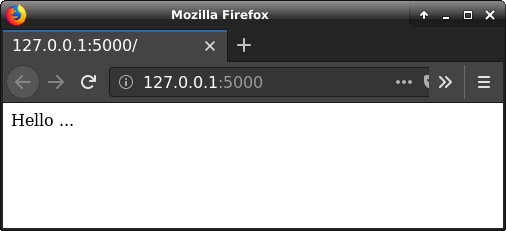
\includegraphics[scale=0.5]{images/Firefox_Hello_v1.png}
\par}
\caption{Tampilan \texttt{ContohFlask}}
\end{figure}

\subsection{Penjelasan kode}

\begin{pythoncode}
from flask import Flask
\end{pythoncode}

Kode ini akan memuat fungsi \texttt{Flask} pada modul \texttt{flask}.
Fungsi \texttt{Flask} digunakan untuk inisialisasi objek \texttt{app}
yang merupakan pengontrol dari website yang akan kita buat.
Inisialisasi objek \texttt{app} dilakukan pada kode berikut ini.
\begin{pythoncode}
app = Flask(__name__)
\end{pythoncode}

Setelah \texttt{app} diinisialisasi, kita perlu membuat fungsi-fungsi
yang akan merespon pada jika ada request yang datang pada webserver.
Pada kode sebelumnya, fungsi ini bernama \texttt{hello} yang akan
merespon jika URL yang diminta adalah root ("/"). Bentuk dasar dari fungsi
ini adalah:
\begin{pythoncode}
@app.route("/link-name")
def nama_fungsi():
    # berikan respon yang sesuai di sini.
\end{pythoncode}
Fungsi inilah yang akan merespon jika ada webserver diakses dengan format
\url{http://alamat_server:nomor_port/link-name}. Secara default nama
\url{alamat_server:nomor_port} yang digunakan pada Flask adalah
\texttt{127.0.0.1:5000}


Sebagai contoh yang kita gunakan sebelumnya.
\begin{pythoncode}
@app.route("/")
def hello():
    return "Hello ..."
\end{pythoncode}

\subsection{Latihan}
Coba tambahkan fungsi berikut ini dalam file \texttt{ContohFlask.py}.
\begin{pythoncode}
@app.route("/about-me")
def about_me():
    return """
    My name is Jono.<br>
    I am a student of MI3103"<br>
    I am learning web development using Flask.<br>
    """
\end{pythoncode}

Restart webserver Anda, kemudian akses \url{http://127.0.0.1:5000/about-me}.
Anda seharusnya akan melihat tampilan seperti ini.
\begin{figure}[h!]
{\centering
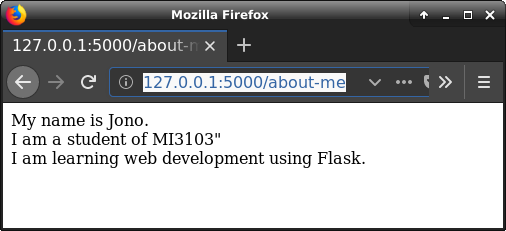
\includegraphics[scale=0.5]{images/Firefox_Hello_v2.png}
\par}
\caption{Tampilan \texttt{ContohFlask}}
\end{figure}

\subsection{Agar dapat diakses dari komputer lain}

Secara default web yang Anda buat hanya dapat diakses dalam komputer Anda sendiri.
Agar dapat diakses dari komputer lain Anda harus menggunakan perintah berikut ini
\begin{textcode}
flask run --host=0.0.0.0
\end{textcode}
atau (jika \texttt{flask} tidak ada dalam \texttt{PATH})
\begin{textcode}
/home/students/anaconda3/bin/flask run --host=0.0.0.0
\end{textcode}

Sekarang coba akses web Anda dari komputer lain dengan menggunakan browser.
Dari komputer tersebut Anda harus mengganti 127.0.0.1 dengan alamat IP komputer
Anda di mana webserver Flask dijalankan.




\end{document}


